\documentclass{cmspaper}
\usepackage{xspace}
\usepackage{verbatim}

\begin{document}
%==============================================================================
% title page for few authors

\begin{titlepage}

% select one of the following and type in the proper number:
%   \cmsnote{2005/000}
  \internalnote{2006/000}
%  \conferencereport{2005/000}
   \date{27 October, 2006}

  \title{Design and Implementation Plan for DBS-2}

  \begin{Authlist}
  Anzar Afaq,  Lee Lueking,  Vijay Sekhri     
\Instfoot{fnal}{FNAL, Batavia, IL, USA}
Andrew Dolgert,  Chris Jones,  Valentin Kuznetsov, Dan Riley
\Instfoot{cornell}{Cornell, Ithaca, NY, USA}

  \end{Authlist}

% if needed, use the following:
%\collaboration{Flying Saucers Investigation Group}
%\collaboration{CMS collaboration}

%  \Anotfoot{a}{On leave from prison}
%  \Anotfoot{b}{Now at the Moon}

  \begin{abstract}
    This is the plan for design and implementation for the second generation DBS system (DBS-2) to replace the existing prototype (DBS-1). It is based on the discussion and material presented at the DBS Workshop held at Cornell in July 2006, and on subsequent work. This document describes the differences between DBS-1 and DBS-2, and describes the schema, API, architecture, and deployment of the new system. A schedule and set of milestones is also included.
 
  \end{abstract} 
  
\end{titlepage}

\setcounter{page}{2}%JPP


%
%==============================================================================

\section{Introduction}

The Dataset Bookkeeping System (DBS) is the component of the CMS data
management system responsible for the site independent description of
the data.  Architecturally, it is built on the concept of a single
``global scope'' DBS at CERN (which could be mirrored read-only for
performance and availability reasons), containing descriptions of all
datasets available to the entire collaboration, and multiple ``local
scope'' DBS instances for particular processing purposes.  Normally
all data files will be recorded initially in a local scope DBS, with
eventual ``publication'' to the global scope DBS where accessibility
throughout the collaboration is required.  Local scope DBS instances
use the same API and schema as the global scope DBS.

This document is based on work that was started at the DBS Workshop at Cornell in July of 2006. Many of the things discussed at the workshop~\cite{dbs-workshop},and followup meetings, are included in the DBS Roadmap~\cite{dbs-roadmap} and it should be consulted for additional information.This plan does not include the data discovery work described in a seperate document. We refer to the project asDBS-2 or ``Cayuga'', named after the Finger Lake near Ithaca. 

\subsection{CMS Data Management Concepts}

\begin{description}
\item{Dataset}-a set of files representing a coherent sample.  Datasets are
defined primarily by processing history and event selection criteria.
\item{Primary Dataset}-Data at all levels of processing pertaining to a given
trigger or common MC production criteria.  For data from the experiment, the
primary dataset is determined by the HLT event classification.
For Monte Carlo data, 'primary datasets' comprise
data generated with the same parameters; the granularity of this
classification has yet to be decided.
\item{Processed Dataset}-A slice of data from a Primary Dataset defined by the
processing history applied to it.  A processed dataset
will correspond to a large production of data with a
single major software release version, but may include
multiple minor versions for small bug fixes and also
may contain the output of multiple processings of
some given input data.
\item{Analysis Dataset}-A subset of a Processed Dataset representing a
coherent sample for physics analysis, 
specified (conceptually) by running an analysis query on a Processed Dataset at
a particular instant of time.  An Analysis Dataset must not contain
the output of multiple processings of any given input data.
\item{Luminosity Section}-''a predefined period of data taking where the
instantaneous luminosity can be considered constant''.  Files intended
for physics analysis will begin and end on luminosity section boundaries.
\item{Data Tier}-A set of objects to be grouped together in the output
files of the processing step producing the objects.  The list of objects
comprising a Data Tier is determined by the release configuration files.
Additional objects not part of the Data Tier may be included in the same
output file.
\item{File Block}-A slicing of a dataset into chunks of files 
likely to be accessed together.  The File Block is a
data management packaging unit for the convenience of the data
location and transfer services.
\item{Logical File Name (LFN)}-globally unique, site independent
file specification suitable for use in job configuration.
\item{Physical File Name (PFN)}-a site-dependent file specification
which can be used to access a file at a particular site.
\end{description}

\subsection{Relationships to CMS Data Management and Workflow Management Areas}


The DBS system is just one component in the Data Management system, and also has relationships to other sources of information in CMS at large. An overall picture of CMS is illustrated in Fig.~\ref{fig:dbs-context-diagram} with DBS represented in the center. Parts of the DBS API/Schema are expanded to more precisely illustrate the relationships with other systems, for example runs and luminosity sections have close associations with many of the data related databases, shown in yellow. Blocks and files have close ties to other parts of the data management system, DLS and PhEDEx, shown in purple. In some cases it may be sufficient for the relationships to be made through the provided APIs for each system. However, it may be much more efficient, i.e. faster, if database links to the various schemas are provided for data that resides in Oracle.

\begin{figure}[hbtp]
  \begin{center}
    \resizebox{15cm}{!}{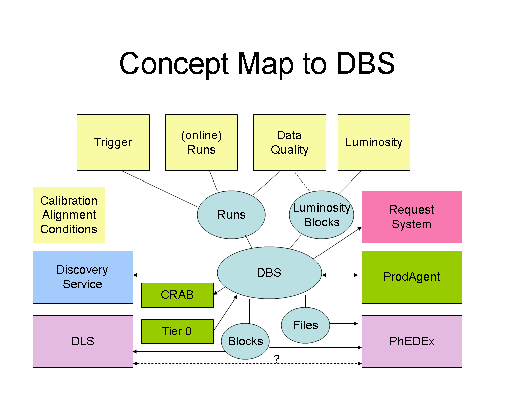
\includegraphics{figure/DBS-WS-DatabasesConceptMap-20060721.eps}}
    \caption{Concept diagram for DBS within CMS.}
    \label{fig:dbs-context-diagram}
  \end{center}
\end{figure} 

\begin{description}
\item{DataSet Location Service (DLS)}--maps File Blocks to storage elements.
It provides only the  names of sites hosting the data and not the physical
location of the constituent files at the sites.
\item{PhEDEx}--data transfer and placement system.
\item{Trivial File Catalog (LFC)}--a site-dependent rules-based file catalog to map LFNs to PFNs.
\item{CRAB}--User analysis job workflow management
\item{ProdAgent}--Monte Carlo production workflow management
\item{EDM Framework}--Event data processing framework
\end{description}

The EDM Framework does not directly interact with the DBS--all
DBS/Framework interactions are mediated by one of the workflow
management tools.  Workflow management is responsible for
configuring the input and output LFNs, which the Framework
maps to PFNs using the LFC.  Information about the output
files is recorded in the Framework Job Report (FJR); the
workflow management system is responsible for registering
the output files in the local DBS/DLS, copying the output to
the appropriate custodial site, and publication to the global
DBS and DLS.

\subsection{Typical Use Cases}

Use cases for the local scope DBS instances include MC and data
production and user data analysis.  In a typical
production scenario, the steps are:

\begin{enumerate}
\item Identify the desired input data via queries to the global DBS
\item Locate the input data via queries to the global DLS
\item Copy the DBS information for the input data to the appropriate
local scope DBS
\item Configure and submit the EDM framework production jobs
\item As jobs finish, collect the framework job reports and register
the intermediate output files into the local scope DBS
\item Merge the intermediate output files into final output files
registered in the local scope DBS
\item Publish the final output files to the global scope DBS
\item Copy the final output files to the appropriate Tier1 and
register with the global DLS
\end{enumerate}

\subsection{Feature Comparison of DBS-1 and DBS-2}

Development of DBS-2 has largely been guided by observations of the
problems (and successes) of SC4 and CSA06, and consideration of the
features that will be required to support physics analysis of CMS
data in the near-term.

The DBS-1 schema included several features that proved to be
problematic, which have been fixed in DBS-2.  The relationship
between Event Collection, File and File Block in DBS-1 was
complicated, largely due to the need to support the FEVT data
tier and old ORCA data.  ORCA data will not be supported in
DBS-2, and FEVT will be supported via a combination of DBS
parentage data and EDM Framework support for processing raw
data and RECO from separate files, so Event Collection has been
removed from the DBS-2 schema and the relationship between
File and File Block simplified.

The DBS-1 schema included an incorrect constraint on the
relationship between Processing (Algorithm/Application
configuration) and Processed Dataset, which forced the
adoption of awkward workarounds during production to
register data produced with the same configuration from
different primary datasets.  This is corrected in DBS-2
with a more general relationship between Algorithm Configuration
and Processed Dataset.

DBS-2 adds support for Primary Dataset descriptions,
and preliminary support for query-able parameter sets,
luminosity sections, and Analysis Datasets (ADS). Primary
datasets can be of types 1. Monte Carlo, 2. Detector Data, 
and 3. Generic. The schema can be updated to accommodate additional 
types as we identify them. Analysis Datasets will be created based on
Definitions that use information  such as application, app version, 
run range, data quality, and other information in the database related 
to lumi blocks and files. ADS Definitions (ADSD) can include or exclude 
data based on these criterion.
A snapshot is provided to insure that an ADS defined at a particular 
time is always reproducible and a warning issued if, for whatever 
reason, this is not the case(e.g. lost files) when it is used. 
% --> add descriptions 

The implementation details for DBS-2 are geared to achieve 
architectural and long-term maintainability goals.  The 
system will be deployable with Oracle or MySQL, and  data 
served to clients in either server or stand-alone modes. 
For the short term, we will not include SQLite but if this 
is needed would consider it when everything else is working. 
The server is written as a Java package and will run as a servlet under 
tomcat with the possibility of using JBOSS if the environment 
it provides is useful down the road. JDBC is used for the database connection
and Tomcat provides connection pooling and management.
 In the stand-alone mode the python client communicates directly with the 
database interface layer (server package).    

\section{DBS Schema}

The complete schema is shown in  Fig.~\ref{fig:new-dbs-schema-design} and described in this section. The up-to-date schema is always available on the web~\cite{dbs-schema}
\begin{figure}[hbtp]
  \begin{center}
    \resizebox{15cm}{!}{\includegraphics{figure/whole_schema_20061025.eps}}
    \caption{New DBS schema design.}
    \label{fig:new-dbs-schema-design}
  \end{center}
\end{figure} 
%	table overview
\subsection{DBS Responsibilities}



The DBS view of CMS data management is ``file-centric''.
For each data file produced or published at the scope of a DBS instance,
the DBS is responsible for recording:

\begin{itemize}
\item LFN, size, checksum, data tier, etc. of the file
\item The ``parent files'' that were input to the job(s)
that created the file
\item The application version and configuration that produced
the file
\item The Processed Dataset of the file
\item The luminosity sections represented in the file (not fully
defined)
\end{itemize}

The DBS also records:

\begin{itemize}
\item Primary Dataset names and descriptions
\item Processed Dataset names, descriptions and parentage
\item Runs, with number of events luminosity sections
\item Luminosity sections with starting and ending event identifiers
\item Analysis Datasets (not fully defined)
\end{itemize}

%	relationships and reasoning

\section{DBS API}

The following is a list of API calls being prepared for the Cayuga (DBS-2) server. We will maintain backward compatibility with existing CRAB, PhEDEx, API functionality. An XML format which includes the data payload is used for client to server communication and is similar to that used in the DBS-1 prototype.
\begin{description}
   \item{listPrimaryDatasets} will take pattern as an input that can be matched against primary dataset name. It will list all the primary datasets along with their descriptions.
   \item{listProcessedDatasets} will take dictionary as an input. The dictionary may contain pattern for path, appVersion, appFamily or appExe. It will list all the processed datasets along with their algorithm information that match either the path and/or application information.
   \item{listApplications} will take dictionary as an input. The dictionary may contain pattern for appVersion, appFamily or appExe. It will list all the applications that match the input pattern
   \item{listRuns} will take path as in input. It will list all the runs within a processed dataset.
   \item{listTiers} will take path as in input. It will list all the tiers within a processed dataset.
   \item{listBlocks} will take path as in input. It will list all the blocks within a processed dataset.
   \item{listFiles} will take dictionary as in input.The dictionary may contain path and/or blockName and/or pattern for lfn.  It will list all the files either in a processed dataset or in a block or in both that match the lfn pattern.
   \item{listDatasetProvenance} needs to be discussed further to understand the logic.
   \item{listDatasetInfo} will take dictionary as an input. The dictionary will contain path for the processed dataset and may or may not contain blockName. It will return a snapshot of the dataset which may be restricted only a single block.
   \item{insertPrimaryDataset} will take dictionary as an input.
   \item{insertApplication} will take dictionary as an input.
   \item{insertBlock} will take dictionary as an input.
   \item{insertProcessedDataset} will take dictionary as an input.
   \item{insertFiles} will take dictionary as an input. The dictionary will include the run information also.
   \item{insertDatasetInfo} will take dictionary as an input.
   \item{closeBlock} will take blockName as in input.
   \item{setFileStatus} will take lfn as an input.
   \item{remapMergedFiles} will take list of lfn and a single lfn as an input.
\end{description}

Several analysisDataset api calls are needed, and are not fully worked out but we can summarize the general needs. The API for ADS will include ability to create the definition, create the timestamped "snapshot", compare two definitionss, or two snapshots, clone and/or modify and validate that all files in an exisitng ADS are calid.





\section{Miscellaneous}
\subsection{Deployment Issues}
We consider deployment issues for each component of the system, specifically the schema, server and client. 
\subsubsection{Schema}
There will be a set of deployment scripts and procedures that are used for both Oracle and MySQL installations. A sql script is needed for both the Oracle and MySQL schema generation. Should share basic schema description and only have technology specific parts separate.
   
\subsubsection{Server}
  Java servlets can be distributed as WAR files for use with Tomcat installations,  or  RPM's for standalone client mode operation. Validation tests that can determine if the system is working once installed and diagnose problems at any time will be provided. The details of the tomcat installation must be clear for local sites such as what ports can be used. A way is needed to monitor the tomcat servers from outside local site. Everything about the local installation needs to be configurable, such as port numbers, oracle or mysql, and so on. Local administrators need to follow the restrictions and policies of the site.


\subsubsection{client}
The client will be distributed through RPMs. Validation tests will be part of the distribution and included in the installation procedure.

\subsection{Global and Local Installations}
 For the CERN Global installation we will plan for a failover configuration that would use at least one high availability server on interruptible power (UPS).If the load warrants multiple machines can be used to scale up with  DNS round robin  set up  similar to that used by the FroNTier system. This system will use the CMS production Oracle database and be a production system with 24/7 hardware support.

Tier-0 should have a so-called ``local'' setup and data will be staged there before it is migrated to the global instance. This instance will be maintained in the CMS production Oracle database at CERN and the system is fully backed up and has 24/7 support.

Local installations at Tier-1 and Tier-N centers are the responsibility of the local site support team. It is believed that these installations, although important, are not as critical as the Global instance. The local instance should be operated in such a manor that  if it  is corrupted or lost only a few hours of work would be lost. Instances where local instances are more critical should be considered on a case-by-case basis and proper attention will be given. 



\subsection{Configuration Management and Version Control}
Maintaining a functioning system overall requires that the schema and code evolves in a  forward and backward compatible way with the adjoining layer. Since the clients are distributed and installed at many locations it is particularly important that incompatibilities be avoided, or made explicitly clear to the user.
We must have an operational matrix of interoperable versions for schema, server, and client.  Each active layer (server and client) will use the version that is actively used by the adjoining layer to determine the proper action or response. The server checks the schema version and is able to deal with minor schema changes.  The client sends it's version with each request and the server is able to deal with each client version, or fail and return a message indicating that the client is incompatible and which minimal version is needed.

   \subsection{Authentication and Authorization}
Authentication and authorization will be provided through Grid Certificates, VOMS and GUMS.
\begin{itemize}
      \item Will use x.509 certificates from the client . A Part of the Globus GSI is used on the server for the authentication.
      \item There will be authorizations for inserting new data, modifying certain status fields, and modifying existing data.
      \item Read only access should not require authentication.
\end{itemize}
   \subsection{Monitoring}
  Monitoring tools similar to those used for the existing prototype will be employed. These include a log analyzer and statistics collector and heartbeat pinger. 
\section{Plan of Work}
The overall plan is to have a working system for Oracle and MySQL by the end of November with full unit tests for the server and client API. In December and the first  part of January we will include additional function for analysis datasets, integrate with ProdAgent and CRAB,  and do performance and stress testing. The system  is expected to be ready for production operation in February 2007.
A time table for the DBS work is shown in Table~\ref{tab:dbs-work-plan}. The manpower includes \~4 FTE from Riley, Kuznetsov, Dolgert, Jones,  Lueking, Afaq, Sekhri. 
\begin{table}[htb]
    \caption{DBS workplan for the Sept. 2006 through Jan. 2007 in detail.  }
    \label{tab:dbs-work-plan}
    \begin{center}
     \begin{tabular}{|l|p{5.5in}|} \hline 
Date & DBS Cayuga  \\ \hline
Sep. 2006 & 
\begin{flushleft} 
1. Use case development.\\ 
2. Schema review and revisions.\\
3. API object and Calls detailed working list and initial users guide.
\end{flushleft} \\ \hline
Oct. 2006  & 
\begin{flushleft}
 1. Schema prototype.\\
 2. Practice deployment to local (MySQL) and global (Oracle) environments.\\ 
 3. API prototyping.\\
 4. Develop unit tests.\\ 
 5. complete design and implementation plan.\\
\end{flushleft}  \\ \hline
Nov. 2006  & 
\begin{flushleft}
 1. Oracle and MySQL deployment details worked out
         a) schema: scripts for schema creation,
         b) server: work out details of the server that are specific to each oracle and mysql,
         c) Testing deployment at Cornell.\\
 2. Unit tests for server.\\
 3. Unit tests for existing client calls.\\
 4. API calls to do:
         a) create primary datasets,
         b) create processed datasets,
         c) create file block,
         d) create algorithm,
         e) insert file,
         f) list primary DS, Files, Processed datasets.\\ 
 5. User documentation, installation, API usage:
         a) JavaDoc? for server,
         b) PyDoc? for client,
         c) Official place for the schema documentation.\\ 
 6. Discovery page compatibility tests with DBS-2.\\
 7. Analysis DS API will begin Mid November.\\
 8. Review of plans in Mid November.\\
 9. Continue development and testing of schema and API.\\
 10.Production server planning.\\
 11.Develop testing and performance benchmarks.\\
\end{flushleft}   \\ \hline
Dec. 2006      & 
\begin{flushleft}
 1. Have local and global fully functional and working together.\\
 2. Complete remaining API work: a) Analysis DS API ready and working,
   b) remap API for merged files,
   c) migration (promotion, publishing) API's,
   d) all other API calls\\
 3. Integration and testing with Discovery tools.\\
 4. Integration with ProdAgent, CRAB, Tier-0 and other CMS tools and Framework. \\
 5. Continued development and testing.\\
 6. Refine production environment.\\  
\end{flushleft} \\ \hline
Jan. 2007  & 
\begin{flushleft} 
 1. Logging and monitoring details implemented.\\
 2. Continued stress testing w/ full estimated load and 2 years datasets.\\
 3. Ready for production operation.\\
 4. Develop procedure for migrating data from DBS-1 as needed.\\
 5. Final documentation and test procedures.\\
 6. Additional discovery and integration with CMS DB areas.\\
 \end{flushleft}    \\ \hline
      \end{tabular}
    \end{center}
  \end{table}  



\begin{thebibliography}{9}
  \bibitem {dbs-workshop} {The DBS Cornell Workshop web site: https://wiki.lepp.cornell.edu/workshops/bin/view/DBSWorkshop/}
  \bibitem {dbs-roadmap} {The DBS Roadmap document:https://twiki.cern.ch/twiki/pub/CMS/DBS-TDR/roadmap.pdf}
  \bibitem{dbs-schema} {Latest schema is at http://home.fnal.gov/~anzar/DBS/DBSSchema/DBSSchemaFridayThe13thOct2006/XHTML/}
  \bibitem {tomcat}{Tomcat home page: http://tomcat.apache.org}

\end{thebibliography}

\end{document}
